\begin{frame}[label=title]
    \centering
    \begin{figure}[H]
        \includegraphics[keepaspectratio, width=0.7\paperwidth, height=.6\paperheight]{Logos/FreeFlower.pdf}
    \end{figure}
    Informatik: Data Science und Sicherheit\\
    \emoji{clamp}\textbf{Kompression}: Intro
\end{frame}

\begin{frame}{Weshalb Kompression? \emoji{clamp}}
	\begin{itemize}
		\item Speicherplatz optimieren
	\end{itemize}
	\begin{figure}[H]
		\centering
		\includegraphics[width=.6\textwidth]{Grundlagen_Info/04_Kompression/Figures/compression3}
	\end{figure}
	\begin{figure}[H]
		\centering
		\raisebox{-0.5\height}{\includegraphics[width=.2\textwidth]{Grundlagen_Info/04_Kompression/Figures/compression1}}
		\raisebox{-0.5\height}{$\rightarrow$}
		\raisebox{-0.5\height}{\includegraphics[width=.25\textwidth]{Grundlagen_Info/04_Kompression/Figures/compression2}}
	\end{figure}
\end{frame}

\begin{frame}{Weshalb Kompression? \emoji{clamp}}
	\begin{itemize}
		\item Speicherplatz optimieren
	\end{itemize}
	\begin{figure}[H]
		\centering
		\raisebox{-0.5\height}{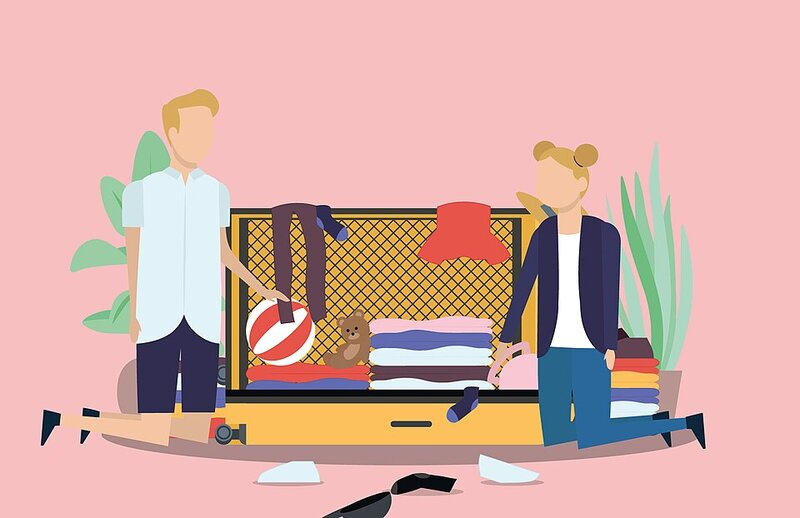
\includegraphics[width=.45\textwidth]{Grundlagen_Info/04_Kompression/Figures/suitcase_messy.jpg}}
		\raisebox{-0.5\height}{$\rightarrow$}
		\raisebox{-0.5\height}{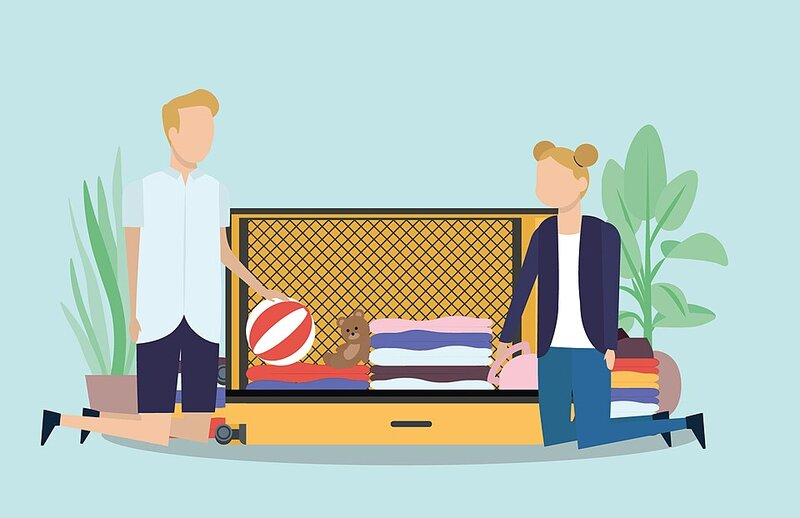
\includegraphics[width=.45\textwidth]{Grundlagen_Info/04_Kompression/Figures/suitcase_packed.jpg}}
	\end{figure}
	{\tiny Bilder: Familydestinationsguide.com Images, \href{https://commons.wikimedia.org/wiki/File:Messy_Suitcase_Packing_for_a_Holiday.jpg}{Wikimedia Commons} und \href{https://commons.wikimedia.org/wiki/File:A_Neatly_Packed_Suitcase_for_a_Holiday.jpg}{Wikimedia Commons}, CC BY 2.0\par}
\end{frame}

\begin{frame}{Weshalb Kompression? \emoji{clamp}}
	\begin{itemize}
		\item Wartezeit verkürzen
	\end{itemize}
	\resizebox{!}{.5\height}{%
	\begin{tikzpicture}
		\path[mindmap,concept color=black,text=white]
		node[concept] {Computer}
		[clockwise from=0]
		child[concept color=green!50!black] {
			node[concept] {Computer}
			[clockwise from=90]
			child { node[concept] {Computer} }
			child { node[concept] {Computer} }
			child { node[concept] {Computer} }
			child { node[concept] {Computer} }
		}
		child[concept color=blue] {
			node[concept] {Computer}
			[clockwise from=-30]
			child { node[concept] {Computer} }
			child { node[concept] {Computer} }
		}
		child[concept color=red] { node[concept] {Computer} }
		child[concept color=orange] { node[concept] {Computer} };
	\end{tikzpicture}}
\end{frame}

\begin{frame}{Kompression: Beispiel}{Römer \emoji{amphora}}
	\begin{itemize}
		\item Pergament und Stein: teure Materialien, deshalb Abkürzungen (z.\,B. SPQR für \textit{Senatus Populusque Romanus})
		\item Römische Zahlendarstellung: z.\,B. Zahl \textbf{999}
		      \begin{center}
			      \texttt{CCCCCCCCCXXXXXXXXXIIIIIIIII}\\
			      $\downarrow$ mit D (500), L (50), V (5)\\
			      \texttt{DCCCCLXXXXVIIII}\\
			      $\downarrow$ Subtraktionsschreibweise: IX, XC, CM\\
			      \texttt{CMXCIX}
		      \end{center}
		\item \texttt{IM} ist keine gültige römische Zahl: I steht nur vor V und X
	\end{itemize}
\end{frame}

\begin{frame}{Verlustfreie vs. verlustbehaftete Kompression}
	\begin{itemize}
		\item \textbf{Verlustfrei}: Original Bit für Bit wiederherstellbar (Texte, Programme, Tabellen)
		\item \textbf{Verlustbehaftet}: lässt weg, was man kaum sieht oder hört (Fotos, Musik, Videos)
	\end{itemize}
	\begin{table}[H]
		\footnotesize
		\begin{tabular}{llll}
			\textbf{Anwendung}  & \textbf{Unkomprimiert}               & \textbf{Verlustfrei}                          & \textbf{Verlustbehaftet}                    \\\midrule
			\textbf{Audio}      & \texttt{.wav} (meist)                & \texttt{.flac}                                & \texttt{.mp3}, \texttt{.aac}                \\
			\textbf{Dateien}    & --                                   & \texttt{.zip}, \texttt{.rar}                  & --                                          \\
			\textbf{Video}      & --                                   & selten                                        & \texttt{.mp4}, \texttt{.mov}, \texttt{.avi} \\
			\textbf{Fotografie} & \texttt{.bmp}, \texttt{.raw} (meist) & \texttt{.png}, \texttt{.psd}, \texttt{.webp}  & \texttt{.jpg}, \texttt{.webp}               \\
			\textbf{Grafik}     & --                                   & \texttt{.svg}, \texttt{.pdf} (Vektorgrafik)   & --
		\end{tabular}
	\end{table}
	{\footnotesize \texttt{.mp4}, \texttt{.mov}, \texttt{.avi} sind Container: Das Video darin komprimiert ein Codec (z.\,B. H.264), meist verlustbehaftet.\par}
\end{frame}

\begin{frame}{Bilder: Beispiel}
	\centering
	\begin{tikzpicture}
		\node[anchor=south west, inner sep=0] (img) {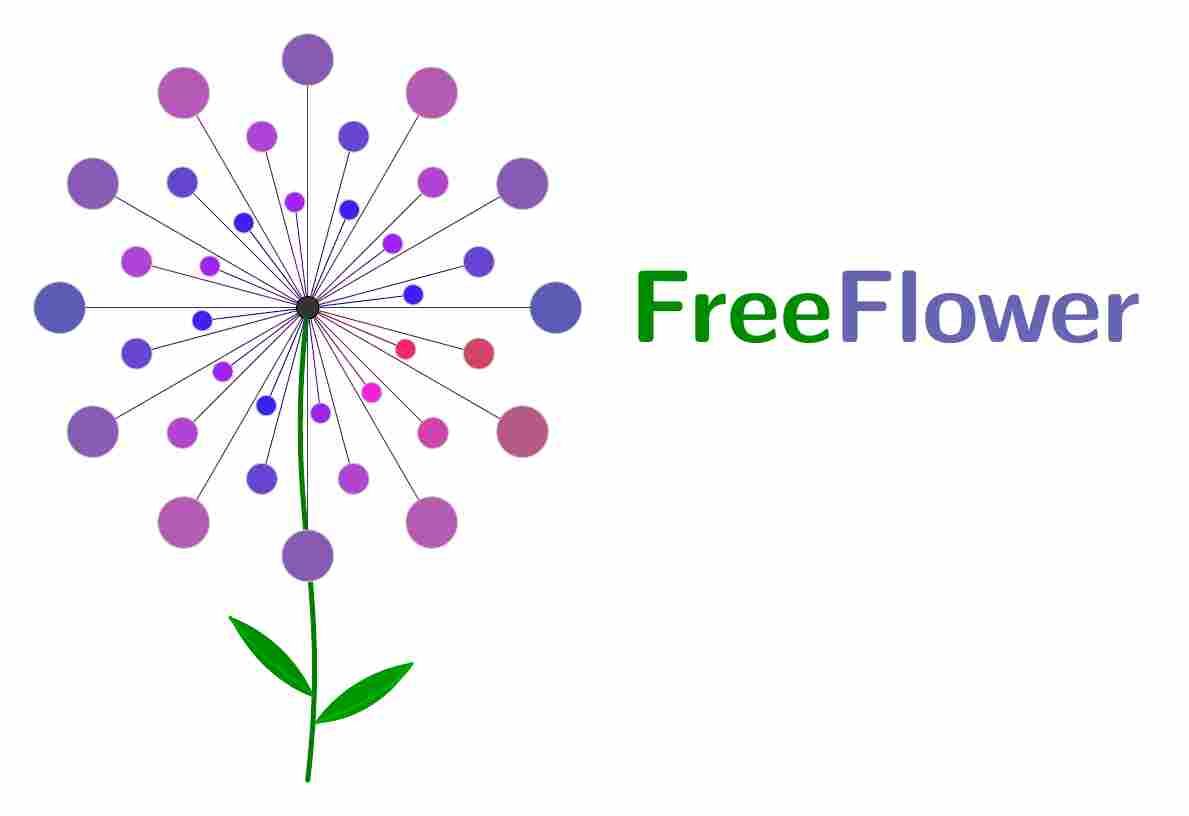
\includegraphics[width=.4\linewidth]{Grundlagen_Info/04_Kompression/Figures/FreeFlowerLogo.jpg}};
		% roter Rahmen = Ausschnitt der Vergrösserung
		\begin{scope}[x=(img.south east), y=(img.north west)]
			\draw[red, thick] (0.538,0.602) rectangle (0.606,0.675);
		\end{scope}
	\end{tikzpicture}\hfill
	\fbox{
\includegraphics[height=.4\textheight]{Grundlagen_Info/04_Kompression/Figures/FreeFlowerLogo_zoom.png}}\\[.5cm]
	\texttt{FreeFlowerLogo\textbf{.jpg}} (21 KB, 300 dpi, starke Kompression)
\end{frame}

\begin{frame}{Bilder: Beispiel}
	\centering
	\begin{tikzpicture}
		\node[anchor=south west, inner sep=0] (img) {\includegraphics[width=.4\linewidth]{Logos/FreeFlower.pdf}};
		\begin{scope}[x=(img.south east), y=(img.north west)]
			\draw[red, thick] (0.538,0.602) rectangle (0.606,0.675);
		\end{scope}
	\end{tikzpicture}\hfill
	% trim in bp: gleicher Ausschnitt wie in FreeFlowerLogo_zoom.png
	\fbox{\includegraphics[height=.4\textheight, clip, trim=153.6 117.8 112.33 63.6]{Logos/FreeFlower.pdf}}\\[.5cm]
	\texttt{FreeFlower\textbf{.pdf}} (9 KB, Vektorgrafik)
\end{frame}

\begin{frame}{Auftrag}
	\begin{itemize}
		\item \aufgabebox{Aufgabe 1.1}
	\end{itemize}
\end{frame}

\begin{frame}{Kompression: Beispiel}
	\centering
	WENN \emoji{blush} HINTER \emoji{blush} $\triangle$, $\triangle$ EINIGE \emoji{blush} ANDEREN \emoji{blush} NACH.

	\only<2>{
		\rule{\linewidth}{.5pt}\\
		\textbf{Auflösung (beispielsweise)}:\\
		WENN GRIECHEN HINTER GRIECHEN RENNEN, RENNEN EINIGE GRIECHEN ANDEREN GRIECHEN NACH.
	}
\end{frame}

\begin{frame}{Kompression: Beispiel}
	\centering
	WENN KLEINE BIENEN HINTER GROSSEN \#3 FLIEGEN, \#1 \#7 \#4 \#6 \#2 NACH.
	\only<2>{
		\rule{\linewidth}{.5pt}\\
		\textbf{Auflösung}:\\
		WENN KLEINE BIENEN HINTER GROSSEN BIENEN FLIEGEN, FLIEGEN KLEINE BIENEN GROSSEN BIENEN NACH.\\[.5cm]
		\#$n$ $=$ dasselbe Wort wie $n$ Wörter weiter vorne\\
		\textbf{Wörterbuchkompression}: Verweise auf Früheres statt Wiederholung (z.\,B. ZIP)
	}
\end{frame}

\begin{frame}{Kompression: LZ77}
	\begin{itemize}
		\item \textbf{LZ77} (Lempel und Ziv, 1977): Verweise auf beliebige Zeichenfolgen statt auf ganze Wörter
		\item Paar (Abstand, Länge): \enquote{Gehen Sie so viele Zeichen zurück und kopieren Sie so viele.}
		\item Kein Wörterbuch nötig: Der bereits dekodierte Text ist das Wörterbuch
	\end{itemize}
	\vspace{.3cm}
	\centering
	\texttt{ANNA UND HANNA} (14 Zeichen)\\[.3cm]
	\only<2>{
		$\downarrow$ ab dem 11.~Zeichen wiederholt sich \texttt{ANNA}, das 10 Zeichen weiter vorne steht\\[.3cm]
		\texttt{A N N A \textvisiblespace{} U N D \textvisiblespace{} H (10,4)}\\[.3cm]
		11 Bausteine statt 14 Zeichen. Verweise lohnen sich erst ab etwa 3 Zeichen.
	}
\end{frame}

\begin{frame}{Auftrag}
	\begin{itemize}
		\item \aufgabebox{Aufgaben 1.2, 1.3}
		\item \challengebox{Aufgabe 1.4}
	\end{itemize}
\end{frame}

\begin{frame}{Kompression: Beispiel}
	\centering
	Wie können wir folgenden Text effizient kodieren?\\[.5cm]
	AACABAAACBACAACADAAD

	\begin{table}[H]
		\begin{tabular}{ccccc}
			\textbf{Buchstabe} & \textbf{A} & \textbf{B} & \textbf{C} & \textbf{D} \\\midrule
			Absolute Häufigkeit & 12 &  2 & 4 & 2 \\
			Relative Häufigkeit & 60\% & 10\% & 20\% & 10\% \\
			\enquote{Naive} Kodierung: & 00 & 01 & 10 & 11 \\
			\enquote{Effiziente} Kodierung: & 0 & 110  & 10&  111\\
		\end{tabular}
		\only<2>{
		\begin{itemize}
			\item \enquote{Naive} Kodierung (40 Bits):\\ \texttt{0000100001000000100100100000100011000011}
			\item \enquote{Effiziente} Kodierung (32 Bits, 20\% Ersparnis):\\ \texttt{00100110000101100100010011100111}

		\end{itemize}
		}

		\only<3>{
		Beide Kodierungen sind \textbf{präfixfrei}: Kein Codewort ist Anfangsstück (Präfix) eines anderen Codeworts}
	\end{table}
\end{frame}

\begin{frame}[fragile]{Codierung als Baumdiagramm}
	\begin{table}[H]
		\centering
			\begin{tabular}{ccccc}
			\textbf{Buchstabe} & \textbf{A} & \textbf{B} & \textbf{C} & \textbf{D} \\\midrule
			Relative Häufigkeit & 60\% & 10\% & 20\% & 10\% \\
			\enquote{Effiziente} Kodierung: & 0 & 110  & 10&  111\\
		\end{tabular}
	\end{table}
	\begin{tikzpicture}
		[-,>=stealth',level distance=15mm,
		level 1/.style={sibling distance=60mm},
		level 2/.style={sibling distance=30mm},
		level 3/.style={sibling distance=15mm},
		level 4/.style={sibling distance=15mm}, leaf/.style={circle, draw}, label/.style={red},edge from parent path={(\tikzparentnode.south) -- (\tikzchildnode)}]


		\usetikzlibrary{shapes}
		\tikzstyle{c} = [draw, shape=circle]
		\tikzstyle{n} = [align=center]
		\tikzstyle{r} = [text=red]

		\node[]{}[edge from parent]
		child {node[n] {A\\ \textcolor{red}{0}}
			edge from parent coordinate (ea);
		}
		child {node[]{}
			child {node[n]{C\\ \textcolor{red}{10}}
				edge from parent coordinate (e25);
			}
			child {node[]{}
				child{node[n]{B\\ \textcolor{red}{110}}
					edge from parent coordinate (e14);
				}
				child{node[n]{D \\ \textcolor{red}{111}}
					edge from parent coordinate (e16);
				}
				edge from parent coordinate (e30);
			}
			edge from parent coordinate (e55);
		};
		% code labels
		\node[r] at([yshift=2mm]ea)  {0};
		\node[r] at([yshift=2mm]e55) {1};
		\node[r] at([xshift=-2mm,yshift=2mm]e25) {0};
		\node[r] at([xshift=2mm,yshift=2mm]e30) {1};
		\node[r] at([xshift=-2mm,yshift=1mm]e14) {0};
		\node[r] at([xshift=2mm,yshift=1mm]e16) {1};
	\end{tikzpicture}
\end{frame}

\begin{frame}{Nicht präfixfrei}
	\begin{itemize}
		\item Kodierung: A $=$ \texttt{0}, B $=$ \texttt{01}, C $=$ \texttt{1}
		\item \texttt{0} ist Präfix von \texttt{01}
		\item Bitfolge \texttt{01}: AC oder B?
	\end{itemize}
	\vspace{.5cm}
	Im Baumdiagramm stehen Buchstaben nur an Blättern: links 0, rechts 1. Der Weg zu einem Buchstaben führt nie über einen anderen Buchstaben, deshalb ist jede Kodierung aus einem Baum präfixfrei.
\end{frame}

\begin{frame}[label=auftrag]{Auftrag}
	\begin{itemize}
		\item \aufgabebox{Aufgaben 1.5--1.7}
	\end{itemize}
\end{frame}
